\documentclass[12pt, a4paper]{article}

\usepackage[utf8]{inputenc}
\usepackage[hmargin=2.5cm,vmargin=2.5cm]{geometry}
\usepackage[brazil]{babel}
\usepackage{graphicx}
\usepackage{amsmath}
\usepackage{steinmetz}
\usepackage{float}
\usepackage{graphicx}


\begin{document}

{\large
\centerline{\textbf{Tarefa 12 - OmpCloud}}
\centerline{\textbf{Introdução à Programação Paralela}}
\centerline{\textbf{Gustavo Ciotto Pinton 117136}}
}

\section{Exercício}

A tabela \ref{tab:resultados}, logo abaixo, contém dados de execuções variando
\(N\) de 100 até 2500 para um \textit{cluster Spark} com 6 nós (2
\textit{masters} e 4 \textit{workers}) criado no sul dos Estados Unidos. Tempos
das execuções \textit{serial} e paralelo estão em segundos.

\begin{table}[h]
    \centering
	\caption{\label{tab:resultados} Resultados obtidos para alguns valores de \(N\).} 
	\begin{tabular}{| c | c | c | c | c | c | }
		\hline
		 & \textbf{100} & \textbf{1000} & \textbf{1500} & \textbf{2000} & \textbf{2500} \\ \hline 
		 Serial (s) & 0.010548 & 6.135442 & 38.299340 & 57.142867 & 189.949704 \\\hline 
		 Paralelo (s) & 65.886165 & 62.775086 & 76.901516 & 126.357308 & 162.322385 \\\hline 
		 Speedup & 0.0003 & 0.097  & 0.498  & 0.452 & 1.170 \\\hline
		
	\end{tabular}
\end{table}

Verifica-se, portanto, que os custos de \textit{offloading} (\textit{download}
e \textit{upload} de dados para/da \textit{cloud}) não justificam o uso do
OmpCloud para valores de \(N\) inferiores a 2500. Evidentemente, tal valor
depende também da qualidade da conexão internet e da localidade das máquinas
criadas no \textit{Azure}.

\vspace{12pt}

A figura \ref{fig:nodes} contém uma captura de tela da interface \textit{web} de
monitoração do \textit{Spark} para a execução com \(N=1000\). É possível
observar, através desta imagem, quais nós foram utilizados para o processamento.

\begin{figure}[h!] 
    \centering
    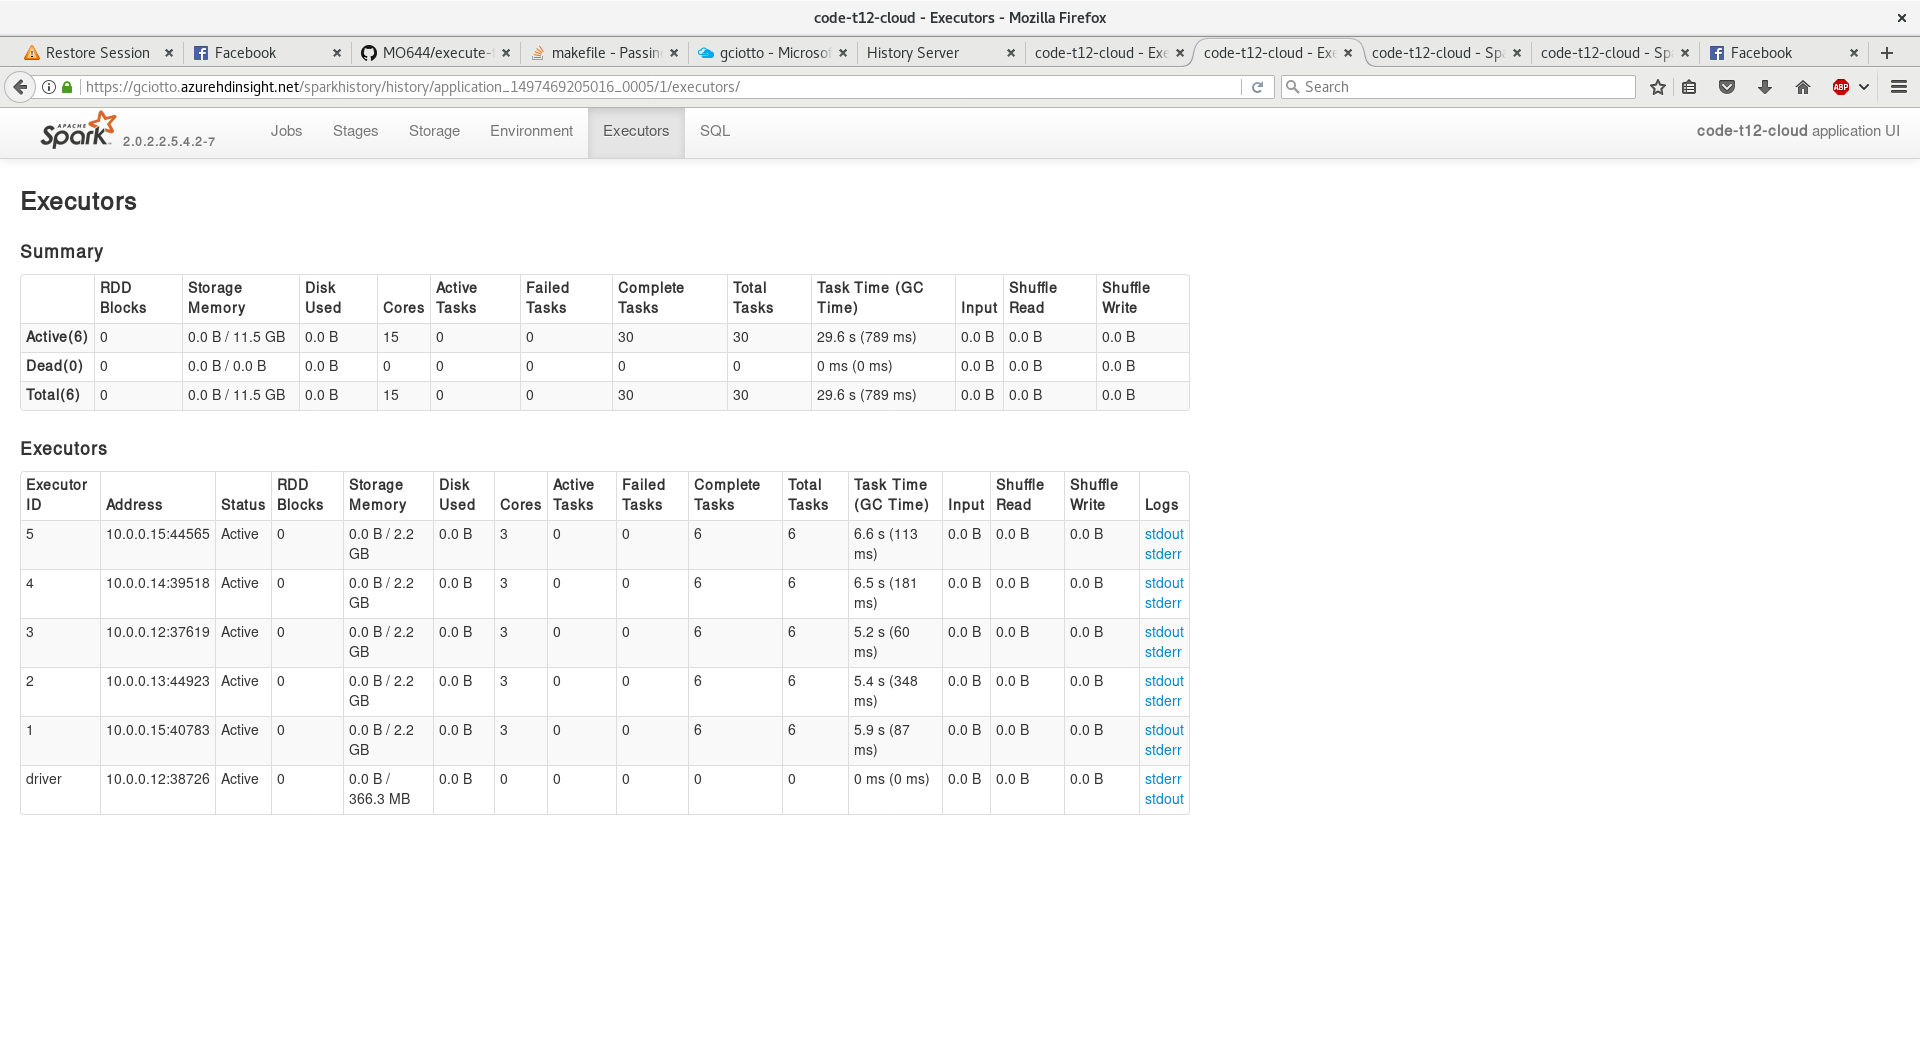
\includegraphics[width=0.96\textwidth]{img/1000/nodes}
    \caption{Divisão das tarefas entre os nós do \textit{cluster}.}        
    \label{fig:nodes}
\end{figure}

Observa-se a presença de 6 nós, conforme esperado. Cinco deles agem como
\textit{executor}, enquanto que o sexto, como \textit{driver} ou
\textit{master}. Conclui-se, portanto, que um dos mestres torna-se um
\textit{worker}, auxiliando, desta forma, nas tarefas de processamento.

\end{document}
